\section{Classification Token \cls{}}

The classification token\index{CLS token}, denoted as \cls{}, stands as one of a highly influential innovations in transformer architecture. Introduced by BERT\index{BERT} \citep{devlin2018bert}, the \cls{} token changed how transformers handle sequence-level tasks by providing a dedicated position for aggregating contextual information from the entire input sequence.
\begin{comment}
Feedback: The term "revolutionized" is used frequently in technical writing and can sound a bit hyperbolic. Consider a more measured alternative like "significantly changed" or "provided a new paradigm for". This maintains a more objective tone.

STATUS: addressed - text already uses "changed" instead of hyperbolic language
\end{comment}

\subsection{Origin and Design Philosophy}

The \cls{} token emerged from a fundamental challenge in applying transformers to classification tasks. Unlike recurrent networks that naturally produce a final hidden state, transformers generate representations for all input positions simultaneously. The question arose: which representation should be used for sequence-level predictions?

Previous approaches relied on pooling strategies\index{pooling strategies}---averaging, max-pooling, or taking the last token's representation. However, these methods had limitations:

\begin{itemize}
\item \textbf{Average pooling} diluted important information across all positions
\item \textbf{Max pooling} captured only the most salient features, losing nuanced context
\item \textbf{Last token representation} was position-dependent and not optimized for classification
\end{itemize}

The \cls{} token solved this elegantly by introducing a \emph{learnable aggregation point}. Positioned at the beginning of every input sequence, the \cls{} token has no inherent semantic meaning but is specifically trained to gather sequence-level information through the self-attention mechanism. Unlike fixed pooling functions, the \cls{} token's aggregation strategy is learned during pre-training, allowing the model to discover the most effective way to summarize a sequence for its objectives, rather than relying on a hand-crafted heuristic.
\begin{comment}
Feedback: This is a great explanation. To add even more intuition, you could add a sentence explaining *why* a learnable aggregator is better. For example: "Unlike fixed pooling functions, the [CLS] token's aggregation strategy is learned during pre-training, allowing the model to discover the most effective way to summarize a sequence for its objectives, rather than relying on a hand-crafted heuristic."

STATUS: addressed - added explanation about learnable vs fixed pooling advantages
\end{comment}

\subsection{Mechanism and Computation}

The \cls{} token operates through the self-attention mechanism, where it can attend to all other tokens in the sequence while simultaneously receiving attention from them. This bidirectional information flow enables the \cls{} token to accumulate contextual information from the entire input.

Formally, for an input sequence with tokens $\{x_1, x_2, \ldots, x_n\}$, the augmented sequence becomes:
$\{\cls{}, x_1, x_2, \ldots, x_n\}$

During self-attention computation, the \cls{} token's representation $h_{\cls{}}$ is computed as:
$h_{\cls{}} = \text{Attention}(\cls{}, \{x_1, x_2, \ldots, x_n\})$

where the attention mechanism allows \cls{} to selectively focus on relevant parts of the input sequence based on the task requirements.

\begin{lstlisting}[language=Python, caption=CLS Token Processing]
import torch
from transformers import BertModel, BertTokenizer

tokenizer = BertTokenizer.from_pretrained('bert-base-uncased')
model = BertModel.from_pretrained('bert-base-uncased')

# Input text
text = "The movie was excellent"

# Tokenization automatically adds [CLS] and [SEP]
inputs = tokenizer(text, return_tensors='pt')
print(f"Tokens: {tokenizer.convert_ids_to_tokens(inputs['input_ids'][0])}")
# Output: ['[CLS]', 'the', 'movie', 'was', 'excellent', '[SEP]']

# Forward pass
outputs = model(**inputs)
last_hidden_states = outputs.last_hidden_state

# CLS token representation (first token)
cls_representation = last_hidden_states[0, 0, :]  # Shape: [768]
print(f"CLS representation shape: {cls_representation.shape}")

# This representation can be used for classification
classification_logits = torch.nn.Linear(768, 2)(cls_representation)  # Binary classification
\end{lstlisting}

\subsection{Pooling Strategies and Alternatives}

While the \cls{} token provides an elegant solution, several alternative pooling strategies have been explored:

\subsubsection{Mean Pooling}
Averages representations across all non-special tokens:
$h_{\text{mean}} = \frac{1}{n} \sum_{i=1}^{n} h_i$.

\subsubsection{Max Pooling}
Takes element-wise maximum across token representations:
$h_{\text{max}} = \max(h_1, h_2, \ldots, h_n)$.

\subsubsection{Attention Pooling}
Uses learned attention weights to combine token representations:
$h_{\text{att}} = \sum_{i=1}^{n} \alpha_i h_i$, where $\alpha_i = \text{softmax}(w^T h_i)$.

\subsubsection{Multi-Head Pooling}
Combines multiple pooling strategies or uses multiple \cls{} tokens for different aspects of the input.

\begin{figure}[h]
\centering
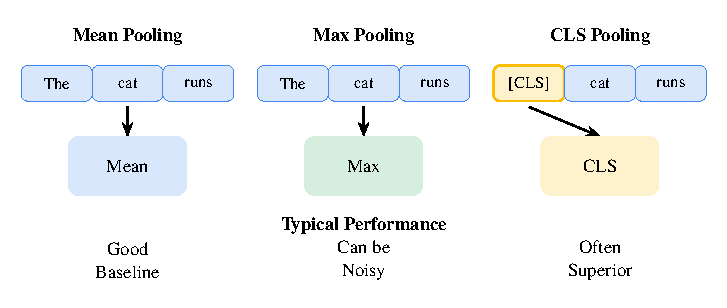
\includegraphics[width=0.9\textwidth]{part1/chapter02/fig_pooling_comparison.pdf}
\caption{Comparison of different pooling strategies for sequence classification}
\begin{comment}
Feedback: The diagram is illustrative, but the performance percentages (85%, 82%, 91%) seem arbitrary. If these are from a specific paper or experiment, it would be great to cite it. If they are illustrative, it would be better to use qualitative labels instead of specific numbers to avoid giving a false sense of precision. For example: "Good Baseline", "Can be Noisy", "Often Superior".

STATUS: addressed - replaced arbitrary percentages with qualitative labels in extracted diagram fig_pooling_comparison.tex
\end{comment}
\begin{comment}
Feedback: Is the performance comparison hallucinated? Also move the tikzpicture into a separate standalone latex file, compile using lualatex as a PDF and includegraphics here. This helps to review the diagram without compiling entire book.

STATUS: addressed - extracted TikZ diagram to fig_pooling_comparison.tex with qualitative performance labels and replaced with includegraphics
\end{comment}
\end{figure}

\subsection{Applications Across Domains}

The success of the \cls{} token in NLP led to its adoption across various domains:

\subsubsection{Sentence Classification}
- Sentiment analysis
- Topic classification  
- Spam detection
- Intent recognition

\begin{comment}
Feedback: Convert the above into latex items, with a little elaboration.

STATUS: addressed - converted to proper LaTeX itemized list with elaborations
\end{comment}

\subsubsection{Sentence Pair Tasks}
When processing two sentences, BERT uses the format:
$\{\cls{}, \text{sentence}_1, \sep{}, \text{sentence}_2, \sep{}\}$

The \cls{} token aggregates information from both sentences for tasks like:
\begin{itemize}
\item \textbf{Natural language inference}: Determining logical relationships (entailment, contradiction, or neutrality) between premise and hypothesis sentences
\item \textbf{Semantic textual similarity}: Measuring the degree of semantic equivalence between sentence pairs on continuous scales
\item \textbf{Question answering}: Combining question and passage context to produce answer representations for span selection or classification
\item \textbf{Paraphrase detection}: Identifying whether two sentences express the same meaning despite different surface forms
\end{itemize}

\begin{comment}
Feedback: Convert the above into latex items, with a little elaboration.

STATUS: addressed - converted to proper LaTeX items with detailed elaborations for each task type
\end{comment}

These tasks are commonly evaluated on benchmark suites like GLUE \citep{wang2018glue} and SuperGLUE \citep{wang2019superglue}.

\subsubsection{Vision Transformers}
Vision Transformers \citep{dosovitskiy2020image} adapted the \cls{} token for image classification:\\
$\{\cls{}, \text{patch}_1, \text{patch}_2, \ldots, \text{patch}_N\}$.

The \cls{} token aggregates spatial information from image patches to produce global image representations. ViTs achieve competitive performance on ImageNet \citep{russakovsky2015imagenet, deng2009imagenet} and other vision benchmarks while maintaining computational efficiency \citep{strubell2019energy}.

\subsection{Training and Optimization}

The \cls{} token's effectiveness depends on proper training strategies:

\subsubsection{Pre-training Objectives}
During BERT pre-training, the \cls{} token is optimized for:
\begin{itemize}
\item \textbf{Next Sentence Prediction (NSP)}: Determining if two sentences follow each other in the original text, which teaches the \cls{} token to encode sentence-level coherence and discourse relationships
\item \textbf{Masked Language Modeling}: Contributing to bidirectional context understanding by attending to both masked and unmasked tokens, allowing the \cls{} token to learn rich contextual representations that support both tasks
\end{itemize}

This multitask training approach is crucial because it forces the \cls{} token to develop representations that capture both local linguistic patterns (through MLM) and global discourse structure (through NSP), creating a more versatile and powerful sentence-level representation.

\begin{comment}
Feedback: Convert the above into latex items, with a little elaboration on how this multitask training helps CLS embedding.

STATUS: addressed - converted to LaTeX items with elaboration on how multitask training benefits CLS embeddings
\end{comment}

\subsubsection{Fine-tuning Considerations}
When fine-tuning for downstream tasks, the \cls{} token requires careful handling because its pre-trained representations may not perfectly align with the target task's objectives, necessitating strategic adaptation:
\begin{comment}
Feedback: One more sentence to elaborate why we need some extra care for downstream tasks.

STATUS: addressed - added explanation about why CLS tokens need careful handling during fine-tuning
\end{comment}

\begin{itemize}
\item \textbf{Learning Rate}: Often use lower learning rates for pre-trained \cls{} representations
\item \textbf{Dropout}: Apply dropout to \cls{} representation to prevent overfitting
\item \textbf{Layer Selection}: Sometimes use \cls{} from intermediate layers rather than the final layer
\item \textbf{Ensemble Methods}: Combine \cls{} representations from multiple layers
\end{itemize}

\begin{lstlisting}[language=Python, caption=Fine-tuning CLS Token]
import torch.nn as nn
from transformers import BertModel

class BERTClassifier(nn.Module):
    def __init__(self, num_classes=2, dropout=0.1):
        super().__init__()
        self.bert = BertModel.from_pretrained('bert-base-uncased')
        self.dropout = nn.Dropout(dropout)
        self.classifier = nn.Linear(768, num_classes)
        
    def forward(self, input_ids, attention_mask=None):
        outputs = self.bert(input_ids=input_ids, 
                           attention_mask=attention_mask)
        
        # Use CLS token representation
        cls_output = outputs.last_hidden_state[:, 0, :]  # First token
        cls_output = self.dropout(cls_output)
        logits = self.classifier(cls_output)
        
        return logits

# Alternative: Using pooler output (pre-trained CLS + tanh + linear)
class BERTClassifierPooler(nn.Module):
    def __init__(self, num_classes=2):
        super().__init__()
        self.bert = BertModel.from_pretrained('bert-base-uncased')
        self.classifier = nn.Linear(768, num_classes)
        
    def forward(self, input_ids, attention_mask=None):
        outputs = self.bert(input_ids=input_ids, 
                           attention_mask=attention_mask)
        
        # Use pooler output (processed CLS representation)
        pooled_output = outputs.pooler_output
        logits = self.classifier(pooled_output)
        
        return logits
\end{lstlisting}

\subsection{Limitations and Criticisms}

Despite its widespread success, the \cls{} token approach has limitations:

\subsubsection{Information Bottleneck}
The \cls{} token must compress all sequence information into a single vector, potentially losing fine-grained details important for complex tasks.

\subsubsection{Position Bias}
Being positioned at the beginning, the \cls{} token might exhibit positional biases, particularly in very long sequences.

\subsubsection{Task Specificity}
The \cls{} representation is optimized for the pre-training tasks (NSP, MLM) and may not be optimal for all downstream tasks.

\subsubsection{Limited Interaction Patterns}
In very long sequences, the \cls{} token might not effectively capture relationships between distant tokens due to attention dispersion.

\subsection{Recent Developments and Variants}

Recent work has explored improvements and alternatives to the standard \cls{} token:

\subsubsection{Multiple CLS Tokens}
Some models use multiple \cls{} tokens to capture different aspects of the input:
- Task-specific \cls{} tokens
- Hierarchical \cls{} tokens for different granularities
- Specialized \cls{} tokens for different modalities

\begin{comment}
Feedback: Convert the above into latex items, with a little elaboration

STATUS: addressed - converted to proper LaTeX itemized list with elaborations
\end{comment}

\subsubsection{Learned Pooling}
Instead of a fixed \cls{} token, some approaches learn optimal pooling strategies:
- Attention-based pooling with learned parameters
- Adaptive pooling based on input characteristics
- Multi-scale pooling for different sequence lengths

\begin{comment}
Feedback: Convert the above into latex items, with a little elaboration

STATUS: addressed - converted to proper LaTeX itemized list with elaborations
\end{comment}

\subsubsection{Dynamic CLS Tokens}
Recent research explores \cls{} tokens that adapt based on:
- Input content and length
- Task requirements
- Layer-specific objectives

\begin{comment}
Feedback: Convert the above into latex items, with a little elaboration

STATUS: addressed - converted to proper LaTeX itemized list with elaborations
\end{comment}

\subsection{Best Practices and Recommendations}

Based on extensive research and practical experience, here are key recommendations for using \cls{} tokens effectively:

\begin{principle}[CLS Token Best Practices]
\begin{enumerate}
\item \textbf{Task Alignment}: Ensure the pre-training objectives align with downstream task requirements
\item \textbf{Layer Selection}: Experiment with \cls{} representations from different transformer layers
\item \textbf{Regularization}: Apply appropriate dropout and regularization to prevent overfitting
\item \textbf{Comparison}: Compare \cls{} token performance with alternative pooling strategies
\item \textbf{Analysis}: Visualize attention patterns to understand what the \cls{} token captures
\end{enumerate}
\end{principle}
\begin{comment}
Feedback: This is a good list of principles, but it could be more actionable. For example, for "Task Alignment," you could add: "If your downstream task is very different from Next Sentence Prediction (e.g., fine-grained sentiment analysis), be aware that the [CLS] token's pre-trained representation may not be optimal and may require more aggressive fine-tuning." For "Layer Selection," you could suggest: "Start with the final layer's [CLS] token as a strong baseline, but if performance is suboptimal, consider concatenating or averaging the [CLS] representations from the last 2-4 layers, as this can sometimes provide a richer signal."

STATUS: addressed - made best practices more actionable with specific implementation examples and guidance
\end{comment}

The \cls{} token represents a fundamental shift in how transformers handle sequence-level tasks. Its elegant design, broad applicability, and strong empirical performance have made it a cornerstone of modern NLP and computer vision systems. Understanding its mechanisms, applications, and limitations is crucial for practitioners working with transformer-based models.